

\documentclass[12pt]{article}         
\usepackage{fullpage}
\usepackage[shortlabels]{enumitem}
\usepackage{amsmath}
\usepackage{amsthm}
\usepackage{graphicx}
\usepackage{amssymb}
\usepackage{enumitem}

\title{250 Homework $\#$4 (Fall  2026)}
\author{Firstname LastName \footnote{Collaborated with Nobody.}}
\begin{document}
\date{}
\maketitle


 This assignment is due at 11:59 p.m.~on  Monday,  9   November 2026, to 
be submitted on Gradescope.  Late assignments (with penalty, unless
excused) will be accepted until
11:59 p.m. on Tuesday,  10 November   2026, and not after.  Please see
the syllabus for more details on homework grading and late penalties.

\medskip

When submitting to Gradescope, please do not forget to assign pages to problems.

%\medskip

% All problems, with the exception of the first two and ,  originally come from the textbook. Some of them have been modified.  In case of doubt, the version printed here is the one you should follow.

\bigskip


The formatting and submission guidelines are the same for this assignment as for the previous ones.  
Please see the Canvas Homework page for the complete  guideline details.




\medskip


 Many of the problems originally come from the textbook and have their original reference numbers, e.g., 4.4.8, attached.   Many of those  have been modified from the book version. In those cases, you should solve the version given here and not the original one in the book.  

% \medskip






\medskip

{\bf Special Induction Rules:} Important. Any problem that requires you   to prove something by induction should be split into three distinct labelled parts:

\begin{itemize}
\item [(i)] State the induction hypothesis $P(x)$ and specify the type of $x.$\\
{\em \small In Q1, this step is already done for you.}

 \item [(ii)] State the  base case(s) and explain why they are correct.

 \item [(iii)] Prove the correctness of the inductive step.\\
    This part  must explicitly show exactly where the induction hypothesis is used in the proof.

\end{itemize}

For reference when doing the problems:


Problems Q1(b), Q2, Q3, Q4, Q5, and Q7(c)  require induction.


Problems Q1(c)  is best done using induction.


Problems  Q1(a), Q6 and Q7 (a) and  do not need induction.

Each of the four parts of the EC should be proven by induction, after stating the appropriate Theorem.
\newpage

\section*{\textbf{Q1. P4.4.8} [10 pts]}
 Pig Floyd is weighed at the beginning of every month. In Month 0 he weighs 400 kilograms, in Month 1 he weighs 350 kilograms, and in later months his weight $W(n + 1)$ is equal to $\sqrt{2}W(n) - W(n - 1) + 700 - 350 \sqrt{2}$.
\begin{enumerate}[(a)]
    \item  Calculate $W(n)$ for all naturals $n$ with $n \leq 10.$\\ Write your answers in the form $W(n) = a_n + b_n \sqrt{2}$ where $a_n$ and $b_n$ are integers.
    
    \item  Prove by strong induction on all naturals $n$ that $W(n)$ can be written in the form $a_n + b_n \sqrt{2}$ where $a_n$ and $b_n$ are integers.\\
    {\em \small For full credit, your induction  proof should be split into parts (i), (ii) and (iii) as described on the first page of this document.}


    \item  Determine $W(84)$, Floyd’s weight after seven years (that is, after 84 months). You might  find it easiest to discover a pattern in the numbers $W(n)$ from part (a)  and then prove that this pattern holds for all $n$ by strong induction. \\
    {\em \small Reminder. If your proof uses  (strong) induction, it should again be split into parts  (i), (ii) and (iii) as described n the first page of this document.}
    
\end{enumerate}

\textit{Note: For part (a) we only want the values a and b.  If you can write a program to find the numbers in the correct $a_n + b_n \sqrt 2$ format, that's fine. Similarly, if you really want to, you can write a program to solve part (c) but, if you do, you must provide a clean, easily readable documented printout of the program as part of your submission with an explanation of why your program is correct. (The proof might be easier than coding it up).
}

\subsection*{\textbf{Solution:}}

\begin{enumerate}[(a)]
    \item  
    \item \ 
        \begin{enumerate}[(i)]
            \item 
            \item 
            \item 
        \end{enumerate}
    \item 
\end{enumerate}

\newpage

\newpage

\section*{\textbf{Q2. For Section 4.7} [10 pts]}


 \noindent A string $w$ is in $B$ if: \\
 \noindent $R_1: w = \lambda.$\\
 $R_2: w = avb$, where $v \in B.$\\
 $R_3: w = uv$, where $u, v \in B$ and $u \neq \lambda, v \neq \lambda.$ \\

 \noindent Let $N_a(w)$ be the number of $a$'s in string $w$.\\
 Let $N_b(w)$ be the number of $b$'s in string $w$.\\
 Let $|w| = N_a(w) + N_b(w)$ be the total number of characters in $w$.\\

 \noindent Prove by induction that, for all strings $w \in B, N_a(w) = N_b(w).$\\ 
 That is, the number of `a's equals the number of `b's.

 \medskip
 
 We will ask you to prove this in two different ways.  The first is by strong induction on the naturals.  The second is by structural induction. \\

 \noindent For both, we will be checking the correctness of the formulations of your logical statement.
 
\begin{enumerate}[(a)]
    \item  For every natural $n$, set the inductive hypothesis $P(n)$ to be the statement that\\ ``For every string $w \in B$ satisfying $|w| \leq n, N_a(w) = N_b(w)$''.\\  Prove correctness of $P(n)$ for all naturals $n$ in the following two steps:

    \begin{enumerate}
        \item[(ii)]What is the base case for induction using $P(n)$? \\ Show that the base case is correct.

        \item[(iii)] Prove the correctness of the inductive step that $P(n) \rightarrow P(n + 1).$
    \end{enumerate}
    
    \item  For every string $w \in B$, set the inductive hypothesis $P(w)$ to be the statement that ``$N_a(w) = N_b(w)$''. Prove correctness of $P(w)$ for all  strings $w$  in the following two steps:

    \begin{enumerate}
        \item[(ii)]  What is the base case for induction using $P(w)$?\\  Show that the base case is correct.

        \item[(iii)]  Given $w \in B$ (and $w$ not the base case), show that $P(w)$ is correct if we assume that every string in $B$ used in the recursive definition of $w$ satisfies $P(w).$
    \end{enumerate}
\end{enumerate}

\subsection*{\textbf{Solution:}}
\begin{enumerate}[(a)]
    \item 
        \begin{enumerate}
        \item[(ii)]
        \item[(iii)]
        \end{enumerate}
       \item 
        \begin{enumerate}
        \item[(ii)]
        \item[(iii)]
        \end{enumerate}     
\end{enumerate}


\newpage
\section*{\textbf{Q3. P4.6.5} [10 pts]}
  {\em Define} the {\em exponentiation operator} on naturals recursively so that $x^0 = 1$ and $x^{S(n)} = x^n \cdot x$. Using this definition:
 
  \begin{itemize}
\item[(a)]  Prove by induction %using this definition, 
  that for any naturals $x, y,$ and $z,$ $x^{y+z} = x^y \cdot x^z$
\item[(b)] Prove by induction %, using this definition, 
  that for any naturals $x, y,$ and $z,$ $x^{y \cdot z} = (x^y)^z.$ 
\end{itemize}


\noindent \textit{Hints: 
\begin{enumerate}
    \item Don't forget to split the induction proof into the three parts, (i), (ii) and (iii).
    \item To prove (b), try replacing $x$ in (a)  by the natural $x^y$.
    \item When trying to prove something is true for three variables, our  standard approach is to arbitrarily fix two of the variables and do induction on the third. For example, in (a), you should  fix $x,y$ and try to prove by induction on $z,$  the proposition $P_{x,y}(z)$, which is  is that ``$x^{y+z}= x^y \cdot x^z$''
    \item You may use any of the known properties of addition and multiplication that we have taught.
    \item As an example, for part (a) (iii) you might start with the assumption $P_{x,y}(z)$ and show that it implies $P_{x,y}(S(z))$, where $S(z)$ is the successor of $z.$ So your proof structure might look something like
    \begin{eqnarray*}
        x^{y + S(z)}  &=& x^{S(y+z)}  \qquad \mbox{Definition of $S(n)$}\\
                      &=&  \ldots\\
                      &\vdots&\\
                    &=& x^y \cdot x^{S(z)}.  
    \end{eqnarray*}
\end{enumerate}
}


\subsection*{\textbf{Solution:}}
\begin{enumerate}[(a)]
    \item \ 
        \begin{enumerate}[(i)]
            \item 
            \item 
            \item 
        \end{enumerate}
    \item \ 
        \begin{enumerate}[(i)]
            \item 
            \item 
            \item 
        \end{enumerate}
\end{enumerate}


\newpage

\section*{\textbf{Q4.  Modification of P4.7.1} [10 pts]}
Let $w$ be  a string over some alphabet $\Sigma.$ Recall that the reversal operator  $w^R$ is defined recursively by (i) $\lambda^R = \lambda$ and, for every string $w,$ and character $a\in \Sigma,$ $(wa)^R = a w^R.$


\begin{itemize}
\item[(a)] Prove by induction on strings that, for every string $w,$ and character $a\in \Sigma,$ $(a w)^R = w^R a.$ 

{\em \small Hint. The end of Lecture 19 proves that for all {\em strings}, $u,v,$  
$(wu)^R = u^R w^R.$ You can modify that proof to solve this}

\item[(b)]  Prove by induction on strings that for any string $w, (w^R)^R = w$.\\
{\em \small Hint. Use part (a).
}

\end{itemize}





\subsection*{\textbf{Solution:}}
\begin{enumerate}[(a)]
    \item \ 
        \begin{enumerate}[(i)]
            \item 
            \item 
            \item 
        \end{enumerate}
    \item \ 
        \begin{enumerate}[(i)]
            \item 
            \item 
            \item 
        \end{enumerate}
\end{enumerate}


\newpage

\section*{\textbf{Q5. Modified P4.11.1} [10 pts]}
Prove  that a $3 \times n$ rectangle can be covered exactly with L-shaped tiles if and only if $n$ is even.  Do this in two parts:

\begin{enumerate}[(a)]
    \item Prove by induction that  if $n$ is even,  then the  board can be tiled.  More explicitly prove that for all natural $n$, a $3 \times (2n)$ can be tiled exactly with $L$-shaped tiles.
    \item Prove by induction that  if $n$ is odd,  then the  board cannot be tiled.  More explicitly prove that for all natural $n$, a $3 \times (2n+1)$ board cannot be tiled exactly with $L$-shaped tiles.
\end{enumerate}


{\em \textbf{Hint}: For (b) it it might help to use an indirect proof, i.e., proof by contradiction. For example, let  $Q(n)$ be the proposition that  a $3 \times (2n+1)$ board cannot be tiled exactly with $L$-shaped tiles. Then, in the inductive step, after assuming $Q(n)$, instead of proving directly that $Q(n) \rightarrow Q(n+1),$ prove instead the equivalent  $\neg Q(n+1)\rightarrow \neg Q(n).$ 
}


\begin{enumerate}[(a)]
    \item \ 
        \begin{enumerate}[(i)]
            \item 
            \item 
            \item 
        \end{enumerate}
    \item \ 
        \begin{enumerate}[(i)]
            \item 
            \item 
            \item 
        \end{enumerate}
\end{enumerate}


\newpage

\section*{\textbf{Q6. P9.1.4} [10 pts]}
 Let $G$ be a tree and let $x$ and $y$ be any two nodes such that $(x, y)$ is not an edge. Let $H$ be the graph obtained from $G$ by adding the edge $(x, y)$. Prove that $H$ has exactly one simple cycle. \\

 \noindent \textit{Hint:  You may use the Unique Path Theorem, taught in class and page 9-3 in the textbook.}

 

\medskip


\subsection*{\textbf{Solution:}}

\newpage

\section*{\textbf{Q7. P9.3.2} [10 pts]}

Recall the definition of the Fibonacci numbers
\begin{equation} \label{eq:9.3.2}
F(n) = \begin{cases} 
      0 & \mbox{if $n=0$} \\
      1 & \mbox{if $n=1$} \\
      F(n - 1) + F(n - 2) & \mbox{if $n>1$}
   \end{cases}.
\end{equation}

Exercise 9.3.2 defines the following Pseudo-Java method that correctly computes the Fibonacci numbers $F(n)$ on any {\bf natural} input $n.$

\begin{verbatim}
    natural fib (natural n) {
         if (n <= 1) 
            return n;
         return fib(n-1) + fib (n-2);
    }
\end{verbatim}

Let $G(n)$ denote the total number of recursive calls are made by the method when called on initial value $n$.   The initial values are $G(0)=G(1)=0$ and $G(2)=2$.

 \begin{enumerate}[(a)]
   

    \item Find an equation describing $G(n)$ by replacing the question marks in the recurrence below with appropriate numbers.  Explain how you derived this from the code.

    \begin{equation} \label{eq:9.3.2b}
    G(n) = \begin{cases} 
      ?? & \mbox{if $n=0$} \\
      ?? & \mbox{if $n=1$} \\
      G(n - 1) + G(n - 2) +  ??& \mbox{if $n>1$}
   \end{cases}.
\end{equation}

     \item  Calculate the values of $G(n)$ for all $n \le 8.$



%For all naturals $n$ with $n \leq 5$, determine how many recursive calls are made by the method of Exercise 9.3.2 on input $n$.

     
     \item  Prove by induction  that, for all $n,$  $G(n) = 2F(n+1) - 2$.
 \end{enumerate}


 \subsection*{\textbf{Solution:}}
 \begin{enumerate}[(a)]
    \item 
    \item
    \item \ 
        \begin{enumerate}[(i)]
            \item 
            \item 
            \item 
        \end{enumerate}
\end{enumerate}


\newpage

\section*{\textbf{Extra Credit:  P9.1.5} [10 pts]}


{\em {\bf Definition:} A rooted tree has degree $k$ if every internal node has $k$ children. 
${\mathcal T}$ will denote the set of all directed trees of degree $k$. }

\medskip

For the purpose of this problem $\mathcal T$ is defined recursively as follows:
\begin{itemize}
    \item The one node tree is in $\mathcal T.$
    \item Tree $T$ is in $\mathcal T$  if $T$ has a root with $k$ children and each of its $k$ children is a tree in $\mathcal T.$
    \item A tree is in $\mathcal T$ only if it can be derived using the first two rules.
\end{itemize}



{\em More Notation: 
use $d(T)$ to denote the depth of $T,$  $L(T)$ to denote the number of leaves in $T$ and $|T|$ to denote the total number of nodes (leaves plus internal nodes) in $T.$ }

\medskip

The diagram shows four $3$-regular rooted trees with their associated depths, number of nodes and leaves.  Note that the root of $T_1$ has three children, all $T_0$ trees.  The root of $T_2$ has three children, the first and third are $T_0$ trees and the second is a $T_1$ tree.

\medskip

    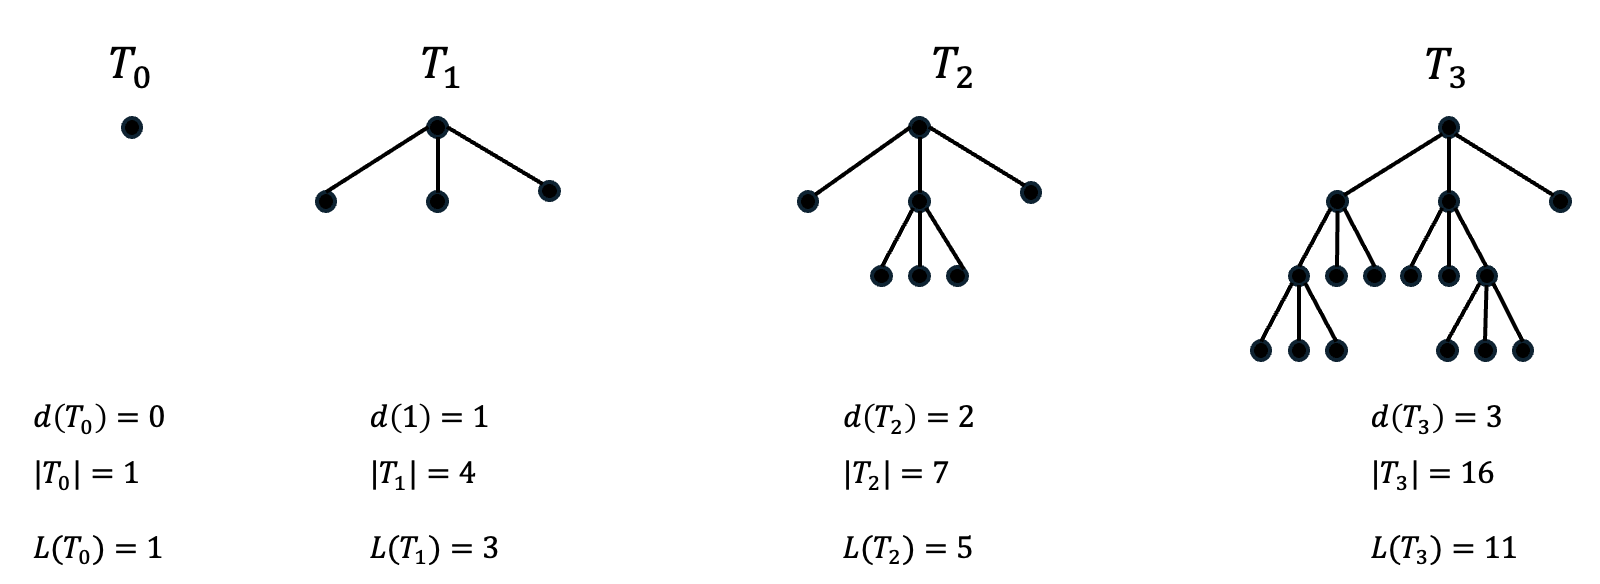
\includegraphics[width=0.8\linewidth]{3_Regular.png}


\medskip
\hrule

\begin{enumerate}[(a)]
    \item State and prove a theorem giving the maximum possible number of leaves  in a rooted tree of depth $d$ and degree $k$.
    \item  State and prove a theorem giving the minimum possible number of leaves  in a rooted tree of depth $d$ and degree $k$.
        \item State and prove a theorem giving the maximum possible number of nodes   in a rooted tree of depth $d$ and degree $k$.
    \item  State and prove a theorem giving the minimum possible number of nodes   in a rooted tree of depth $d$ and degree $k$.
\end{enumerate}

Note: each of these proofs should be done in two parts. In the first part, a bound should be proven by induction.  In the second, the bound should be proven tight.

\medskip

For example, in (a) you should find a function $f(d,k)$ and prove by induction that the number of leaves in  a rooted tree of depth $d$ and degree $k$ is at most $f(d,k).$ An induction proof is  necessary here since the trees are defined recursively.  You should then, for each $d,k$, describe a tree that meets those bounds.

\subsection*{\textbf{Solution:}}
\begin{enumerate}[(a)]
    \item
    \item 
    \item 
    \item
\end{enumerate}

\newpage

\end{document} 